\documentclass{article}
\usepackage{graphicx}
\usepackage{amsmath}
\usepackage{ragged2e}
\graphicspath{ {./figures/} }

\title{TP MATLAB : Transformée de Fourier}
\date{9 Janvier 2021}
\author{Lucas LOISEAU \\ Alexandre SENOUCI \\ Maya BROYER \\ Lena BELIAZI}

\begin{document}
\maketitle
\section{Transformée de Fourier discrète}
Les signaux sont représentés sur l'intervalle $[-5,5]$. \\
On fixe le nombre d'échantillons à $N=32768$. \\
La période d'échantillonage vaut donc $T_e = 3,0518 * 10^{-4}$ et la fréquence d'échantillonage $f_e=3276,8$.
\subsection{Echantillonage et spectre de fonctions usuelles}
\subsubsection{Fonction constante}
On considère la fonction $x_0(t)=42$ dont la transformée de Fourier théorique est $X_0(f)=\delta(f)$, il s'agit d'un nombre réel donc nous affichons uniquement la partie réelle de la transformée de Fourier calculée numériquement.
\begin{figure}[h]
\includegraphics[scale=0.5]{fig_const}
\centering
\end{figure}
\subsubsection{Fonction cosinus}
On considère la fonction $x_1(t)=\cos(2\pi f_0 t)$ avec $f_0=4$, sa transformée de Fourier théorique est $X_1(f)=\frac{1}{2}[\delta(f-f_0)+\delta(f+f_0)]$, il s'agit d'un nombre réel.

\begin{figure}[h]
\includegraphics[scale=0.63]{fig_cos}
\centering
\end{figure}

\subsubsection{Fonction sinus}
On considère la fonction $x_2=\sin(2\pi f_0 t)$ avec $f_0=4$, sa transformée de Fourier théorique est $X_2(f)=\frac{1}{2j}[\delta(f-f_0)-\delta(f+f_0)]$, il s'agit d'un imaginaire pur.
\begin{figure}[h]
\includegraphics[scale=0.6]{fig_sin}
\centering
\end{figure}

\subsubsection{Fonction pic de Dirac}
On considère la fonction $x_3(t)=\delta(t-\Delta t)$, sa transformée de Fourier théorique est $X_3(f)=e^{-j2\pi f\Delta t}$. \\
Lorsque $\Delta t$ est nul, nous constatons bien que la transformée de Fourier du Dirac est constante à $1$ :
\begin{figure}[h]
\includegraphics[scale=0.6]{fig_dirac_0}
\centering
\end{figure} \\
Tandis qu'avec un décalage temporel $\Delta t$ non nul, nous obtenons les courbes suivantes :
\begin{figure}[h]
\includegraphics[scale=0.6]{fig_dirac_deltat}
\centering
\end{figure} \\
Ce qui correspond bien à $Re(X_3(f))=\cos(2\pi f\Delta t)$ et $Im(X_3(f))=\sin(2\pi f\Delta t)$

\subsubsection{Exponentielle complexe}
On considère la fonction $x_4=e^{j2\pi f_0 t}$ qui a comme transformée de Fourier théorique $X_4=\delta(f-f_0)$.
\begin{figure}[h]
\includegraphics[scale=0.6]{fig_exp}
\centering
\end{figure} \\
La transformée de Fourier donne bien $\delta(f-f_0)$ (avec $f_0=4$ sur cette figure).

\subsubsection{Foncion rectangle}
\paragraph{Fonction rectangle apériodique}
Nous allons analyser la fonction rectangle dont la transformée de Fourier théorique est un sinus cardinal.
\begin{figure}[h]
\includegraphics[scale=0.6]{fig_rect}
\centering
\end{figure}
\paragraph{Fonction rectangle périodique}
Nous considérons cette fois une fonction rectangle rendue périodique.
\begin{figure}[h]
\includegraphics[scale=0.6]{fig_rect_per}
\centering
\end{figure} \\
La transformée de Fourier donne cette fois un sinus cardinal discrétisé.
\subsubsection{Courbe de Gauss}
La dernière fonction que nous allons analyser est une courbe de Gauss dont l'équation est $x_6(t)=\exp(-\pi t^2)$
\paragraph{Calcul de la transformée de Fourier théorique}
$$X_6(f) = \int_{-\infty}^{\infty}e^{-\pi t^2}e^{-j2\pi ft}dt=\int_{-\infty}^{\infty}e^{-(\pi t^2 +j2\pi ft)}dt$$. \\
On pose alors
$$\left\{\begin{array}{l}
a^2=\pi t^2 \\
2ab = j2\pi ft
\end{array}\right.
\Rightarrow
\left\{
\begin{array}{l}
a^2=\pi t^2 \\
b^2=-\pi f^2
\end{array}
\right.
$$
L'intégrale se réécrit
$$\int_{-\infty}^{\infty}e^{-(a^2+2ab+b^2)+b^2}dt=\int_{-\infty}^{\infty}e^{-(a+b)^2+b^2}dt$$
On effectue le changement de variable $X=a+b=\pm(\sqrt{\pi}t + j\sqrt{\pi}f)$ avec $\frac{dX}{dt}=\pm \sqrt{\pi}\Leftrightarrow dt=\frac{dX}{\pm\sqrt{\pi}}$ \\
Ce qui donne
$$\int_{-\infty}^{\infty}e^{-X^2-\pi f^2}\frac{dX}{\pm\sqrt{\pi}}=\frac{1}{\pm\sqrt{\pi}}e^{-\pi f^2}\int_{-\infty}^{\infty}e^{-X^2}dX=\pm e^{-\pi f^2}$$
En admettant que $\int_{-\infty}^{\infty}e^{-x^2}dx=\sqrt{\pi}$
\paragraph{Calcul de la transformée de Fourier avec MATLAB}
Nous obtenons le spectre suivant :
\begin{figure}[h]
\includegraphics[scale=0.52]{fig_gauss}
\centering
\end{figure}
\section{Echantillonage et repliement de spectre}
On se propose d'étudier la famille de fonctions paramétriques 
$$g_f(t)=\sin(2\pi f t)+\sin(2\pi(f+\Delta f)t)+\sin(2\pi(f+2\Delta f)t)+2\sin(2\pi(f+3\Delta f)t)$$

avec $\Delta f=50$
\subsection{Calcul des spectres théoriques de $g_{1000}$ et $g_{2250}$}
En exploitant la linéarité de la transformée de Fourier ainsi que le résultat $\sin(2\pi f_0 t)=\frac{1}{2j}[\delta(f-f_0)-\delta(f+f_0)]$, nous obtenons : \\
$$G_{1000}=\frac{1}{2j}[\delta(f-1000)-\delta(f+1000)+\delta(f-1050)-\delta(f+1050)+\delta(f-1100)$$
\flushleft
$$-\delta(f+1100)+2\delta(f-1150)-2\delta(f+1150)]$$
$$G_{2250}=\frac{1}{2j}[\delta(f-2250)-\delta(f+2250)+\delta(f-2300)-\delta(f+2300)+\delta(f-2350)$$
\flushleft
$$-\delta(f+2350)+2\delta(f-2400)-2\delta(f+2400)]$$
\newpage
\subsection{Spectres avec échantillonage}
Pour la fonction $g_{1000}$, nous obtenons le spectre suivant :
\begin{figure}[h]
\includegraphics[scale=0.5]{fig_g1}
\centering
\end{figure} \\
Cela correspond à nos attentes, nous retrouvons bien des pics de fréquence aux valeurs $\pm1000$, $\pm1050$, $\pm1100$ et $\pm1150$.
En revanche, pour la fonction $g_{2250}$, les pics de fréquences obtenus sont incorrects :
\begin{figure}[h]
\includegraphics[scale=0.5]{fig_g2}
\centering
\end{figure} \\
Cela s'explique par le fait que la fréquence maximale du signal $f_{max}=2400\,\mathrm{Hz}$ soit supérieure à la moitié de la fréquence d'échantillonage $f_e=3276,8 \,\mathrm{Hz}$. Un phénomène de repliement de spectre se produit alors et cause l'apparition de fréquences parasites dans le signal.
\section{Transmission par modulation d'amplitude}
\subsection{Opération de modulation sur deux signaux}
\subsubsection{Signaux étudiés}
Nous allons moduler les deux signaux suivants :
$$ s_1(t) = \sum_{n=1}^{10}n\cos(2\pi.10n.t)$$
\begin{figure}[h]
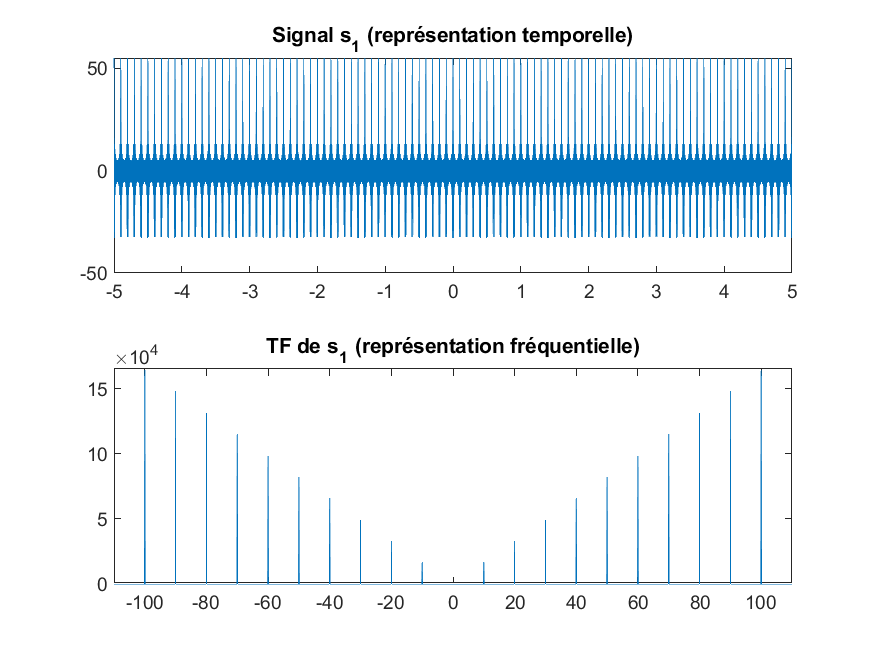
\includegraphics[scale=0.5]{fig_s1}
\centering
\end{figure}
$$ s_2(t)=\sum_{n=1}^{10}(11-n)\cos(2\pi.10n.t)$$
\begin{figure}[h]
\includegraphics[scale=0.5]{fig_s2}
\centering
\end{figure}

\subsubsection{Opération de modulation}
Nous allons maintenant calculer le signal modulé $m(t)$ ayant la propriété de contenir tous les signaux $s_i(t)$. Voici son expression :
$$m(t)=\sum_{i}s_i(t).\cos(2\pi f_i t)$$
Les fréquences $f_i$ propres à chaque signal $s_i(t)$ sont appelées fréquences porteuses. \\
Nous obtenons le résultat suivant pour $m(t)$ avec les signaux $s_1(t)$ et $s_2(t)$ vus précédemment portés par des fréquences $f_1=200$ et $f_2=500$ :
\begin{figure}[h]
\includegraphics[scale=0.6]{fig_modulation}
\centering
\end{figure}
\paragraph{}
Nous observons que le signal modulé en représentation fréquentielle contient les deux signaux centrés autour de leurs fréquences porteuses (et leurs opposés).

\subsubsection{Opération de démodulation}
Nous allons maintenant démoduler le signal $m(t)$ dans le but d'extraire un des signaux qu'il contient. \\
En régle générale, le signal démodulé $d_i(t)$ associé à un signal $s_i(t)$ s'exprime ainsi :
$$d_i(t)=m(t)\cos(2\pi f_i t)$$
\newpage
Voyons maintenant comment un signal $s_i(t)$ transparaît dans son démodulé respectif. Nous avons ici le spectre de $d_1(t)$ :
\begin{figure}[h]
\includegraphics[scale=0.5]{fig_d1}
\centering
\end{figure}
Nous pouvons constater que le signal initial $s_1(t)$ se retrouve avec une amplitude diminuée pour les fréquences inférieures à $100\,\mathrm{Hz}$. Nous pouvons donc l'extraire en appliquant un filtre passe-bas au signal $d_1(t)$.

\subsubsection{Précautions nécessaires pour éviter que les signaux diffusés se mélangent}
\paragraph{}
Dans l'exemple que nous avons étudié, nous avons pu constater que les signaux modulés $s_i(t)$ apparaissaient dans le signal centrés sur leur fréquence porteuse. C'est-à-dire que le signal se retrouvait en symétrie horizontale par rapport à l'axe $x=f_i$. Un signal modulé occupe donc d'après nos observations la bande de fréquences $[f_i-f_{max},f_i+f_{max}]$ avec $f_{max}$ la fréquence maximale de ce signal.
\paragraph{}
Pour éviter que les signaux se chevauchent, nous allons donc vouloir qu'au sein du signal modulé, les fréquences porteuses deux à deux aient une différence supérieure à la somme des fréquences maximales de leur signaux respectifs.
\newpage
Voici un cas limite avec le signal modulé étudié précédemment, où $s_1(t)$ et $s_2(t)$ sont sur le point de se superposer :
\begin{figure}[h]
\includegraphics[scale=0.7]{fig_modulation_limite}
\centering
\end{figure}
\paragraph{}
Nous avons utilisé $f_1=200\,\mathrm{Hz}$ et $f_2=401\,\mathrm{Hz}$ étant donné que la fréquence maximale de $s_1(t)$ et de $s_2(t)$ vaut $100\,\mathrm{Hz}$

\section{Filtrages}
\paragraph{}
\justifying
A partir de la première partie, nous pouvons nous rendre compte qu'il est possible de construire des fonctions de transferts de filtre très utilisés en pratique. Plaçons-nous dans un espace fréquentiel 2D dont les axes seraient u et v, le filtre correspondant au filtrage d'une image 2D serait de la forme de :

\paragraph{}
\centering $H(u,v) = \exp(-K*(u^2+v^2))$
\paragraph{}
où K est une constante permettant de paramétrer les effets du filtre.

\subsection {Les effets du filtre sur l'image selon la valeur de K}
\paragraph{}
\justifying
En créant ce filtre et en l’appliquant à la matrice représentant l’image que l’on veut traiter, il est possible d’appliquer ce filtre à notre image.
En effet, en faisant plusieurs tests sur la valeur de K on peut remarquer plusieurs choses :
\begin{itemize}
\item Plus la valeur de K augmente, plus l’image est floue. Si K est très grand, soit plus grand que 0.5, l’image devient complètement noire, soit aucune fréquence ne passe à travers le filtre, il les bloque toutes.
\item Plus la valeur de K diminue, plus l’image est nette et les bruits sont diminués. En effet, l’image n’est pas plus détaillée, mais plus ‘lisse’. On obtient une bonne représentation de l’image à K = 0.00005.
\item Si on trace la courbe représentant la fonction de transfert H, on voit que c’est une cloche. La largeur de la cloche diminue plus K augmente, et s’élargit plus K diminue. Elle atteint une limite d’une largeur entre [0,1000].
\item On peut aussi remarquer que si K est très petit, se rapprochant fortement de 0, la courbe de fonction de transfert devient un trait horizontal à 1. C’est donc une fonction qui laisse toutes les fréquences entre 0 et 1000 passer. C’est donc un filtre permettant d’ignorer les fréquences hors de ces bornes, mais laisser passer toutes les autres (amplitude = 1).
\end{itemize}
\begin{figure}[h]
\includegraphics[scale = 0.7] {fig_filtre1}
\centering
\caption{La fonction de transfert du filtre utilisée et l'image traitée avec K = 0.00005}
\end{figure}
\begin{figure}
\includegraphics[scale = 0.7]{fig_filtre2}
\centering
\caption {La fonction de transfert du filtre utilisé et l'image traitée avec un K très petit}
\end{figure}
\begin{figure}
\includegraphics[scale = 0.7]{fig_filtre3}
\centering
\caption {La fonction de transfert du filtre utilisé et l'image traitée avec un K très grand}
\end{figure}
\paragraph{}
\newpage
\justifying
On remarque donc que cette fonction de transfert possède la forme du filtre gaussien. Grâce à nos observations nous pouvons conclure que ce filtre permet de réduire les bruits, et donc de ‘lisser’ l’image. 
\paragraph{}
En effet, dépendant de K on peut soit flouter l’image ou la lisser et effacer les bruits extérieurs. Plus K est grand, plus la largeur de la cloche de la fonction gaussienne est petite, moins de fréquences passent et donc plus l’image est floue. Au contraire, plus K est petit, plus la largeur de la cloche est grande et plus les fréquences peuvent passer (donc l’image est plus nette). Quand K est vraiment petit, on atteint une limite et il se rapproche d’un filtre idéal (toutes les fréquences passent et sont d’amplitude 1). 
\paragraph{}
On peut donc penser que ce filtre nous permet donc de réduire les bruits ou de fabriquer une image utilisée pour faire un $ masque flou $.
\subsection{Sous-echantillonner l'image à traiter}
\paragraph{}
\justifying
Lors d’un traitement d’une image, il se peut que celle-ci prenne beaucoup de place. Il est parfois préférable de diviser cette image en 4, soit de la sous-échantillonner en prenant un point sur 4 dans l’image. 
\paragraph{}
Cependant, cette méthode serait peu efficace car très peu représentative de la couleur actuelle des points. En prenant seulement un point sur 4, il serait difficile de reconstituer l’image telle quelle car on ne retrouverait pas du tout les mêmes couleurs. Il y aurait donc une forte dégradation de la représentation de l’image.
\paragraph{}
On pourrait recourir au filtre moyenne, qui remplace chaque pixel par la moyenne des valeurs des pixels adjacents et du pixel central. Ainsi, en prenant un point sur 4, on prendrait en fait un point qui aurait la moyenne des 4 points adjacents, ce qui serait beaucoup plus réaliste lors de la représentation de l’image.


\newpage
\section{Localisation de formes par Corrélation}
\subsection{Méthode de localisation}
\paragraph{}
\justifying
Dans cette partie, nous cherchons à localiser dans une image bruitée trois formes définies. Pour ce faire, nous allons utiliser une localisation par corrélation spatiale. Il s’agit de réaliser toutes les superpositions possibles de ces trois formes sur l’image de référence par translation, en déterminant à chaque fois le taux de ressemblance. Ce-dernier est maximum quand la correspondance est bonne pour une translation donnée. 
\paragraph{}
Pour un signal 2D discret, le taux de ressemblance pourra être calculé à partir de la formule : 
$$Corr(l,c) = \sum_{n=i}\sum_{n = j} S(i,j).F(l+i,c+j)$$
\paragraph{}
\justifying
Où S et F sont respectivement les matrices de couleurs qui représentent la forme à rechercher et l’image bruitée, et l et c deux paramètres spatiaux. 
\paragraph{}
Or, le calcul de la corrélation entre les deux signaux étant similaire à celui du produit de convolution, on préfèrera mesurer la ressemblance par la formule : 
$$Conv(l,c) = \sum_{n=i}\sum_{n = j} S(i,j).F(l-i,c-j)$$
\paragraph{}
\justifying
On remarquera en effet l’équivalence entre le calcul du produit de convolution dans la version spatiale et le calcul du produit simple dans l’espace fréquentiel, beaucoup plus efficace que la première formule proposée. 
\subsection{Réalisation sur matlab}
\paragraph{}
\justifying
On commence par encoder en dur les trois formes à rechercher avec des valeurs numériques : la couleur noire est représentée par la valeur 0 et la couleur blanche par la valeur 1. On complète les matrices avec des 0 pour qu’elles aient la même taille que la matrice représentant l’image de référence (1024*1024), car on effectue la corrélation sur des matrices de même taille. 
\paragraph{}
\justifying 
	On calcule la transformée de Fourier des matrices représentant les formes à rechercher $(F_NEG)$ et l’image de référence (IM) pour obtenir leur représentation fréquentielle à l’aide de la fonction fft2, puis on réalise le produit terme à terme des matrices. On applique ensuite la transformée de Fourier inverse (fonction ifft2) sur la matrice resultat ainsi obtenue, et on réalise une mise à l’échelle pour que l’image en niveau de gris soit codée avec des valeurs entre 0 et 255. La variable compteur représente le nombre d’occurrences de la forme définie dans l’image bruitée. Elle est incrémentée de 1 chaque fois que l’indicateur de ressemblance est suffisamment élevé, c’est-à-dire pour chaque coefficient de la matrice resultat supérieur à 250.  
\begin{figure}
\includegraphics[scale = 0.7]{fig_corr}
\centering
\caption {Localisation de formes par corrélation}
\end{figure}
\subsection{Résultats}
\centering
\begin{tabular}{|c||c|}
        \hline
        Forme à retrouver & Nombre d'occurences \\ 
        \hline
        F1 & 1371\\ 
        \hline
	  F2 & 1322\\
        \hline
	  F3 & 1403\\
	 \hline
\end{tabular} 
\flushleft
\subsection {Avantages et limitations}
\justifying
Cette méthode de localisation des formes, bien que précise et rapide, présente certaines limitations. En effet, elle fonctionne uniquement si la forme à rechercher et l’image de référence se superposent parfaitement. Si on change juste un pixel à cette forme, elle ne sera plus reconnue. Il en va de même si la forme ou l’image bruitée a subi une transformation telle qu’une rotation ou un changement d’échelle. 


\end{document}